\documentclass[specialist, substylefile = spbu_report.rtx, subf,href,colorlinks=true, 12pt]{disser}

\usepackage[a4paper, mag=1000, includefoot, left=3cm, right=1.5cm, top=2cm, bottom=2cm, headsep=1cm, footskip=1cm]{geometry}

\usepackage[T2A]{fontenc}
\usepackage[utf8]{inputenc}
\usepackage[english,russian]{babel}

\usepackage{amsmath}
\usepackage{amssymb}
\usepackage{bbm}
\usepackage{caption}
\usepackage{subcaption}
\usepackage{algorithm}
\usepackage{algpseudocode}
\usepackage{lscape}
\usepackage{graphicx}
\usepackage{dsfont}

\usepackage[unicode, pdftex]{hyperref}

\ifpdf\usepackage{epstopdf}\fi



\DeclareMathOperator{\RE}{RE}
\DeclareMathOperator{\runif}{runif}
\DeclareMathOperator{\Bin}{Bin}
\DeclareMathOperator{\Var}{Var}

\newtheorem{mydef}{Определение}
\newtheorem{theorem}{Теорема}
\newtheorem{designation}{Обозначение}

\newcommand{\ds}{\displaystyle}

\def\letus{%
	\mathord{\setbox0=\hbox{$\exists$}%
		\hbox{\kern 0.125\wd0%
			\vbox to \ht0{%
				\hrule width 0.75\wd0%
				\vfill%
				\hrule width 0.75\wd0}%
			\vrule height \ht0%
			\kern 0.125\wd0}%
	}%
}


\begin{document}

%
% Титульный лист на русском языке
%

% Название организации
\institution{%
	Санкт-Петербургский государственный университет \\
	Прикладная математика и информатика \\
}

\title{Отчет о научно-исследовательской работе}

% Тема
\topic{\normalfont\scshape%
	Применение цепей Маркова в анализе данных}

% Автор
\author{Саттаров Никита Дмитриевич}
\group{группа 19.Б04-мм}

% Научный руководитель
\sa       {Н.\,Э.~Голяндина}
\sastatus {к.\,ф.-м.\,н., доцент}



% Город и год
\city{Санкт-Петербург}
\date{\number\year}

\maketitle

\intro

В книге~\cite[Гл. 6]{stirzaker1992probability} вводится следующее определение цепи Маркова:
\begin{mydef}\label{eq:eq1}
	Конечная последовательность дискретных случайных величин $\{X_{n}\}_{n \geq 0}$ называется конечной цепью Маркова, если
	\begin{equation}
	\mathbb{P}(X_{n+1}=i_{n+1} \mid X_{n} = i_{n}, X_{n-1} = i_{n-1}, \ldots , X_{0} = i_{0}) = \mathbb{P} (X_{n+1}=i_{n+1} \mid X_{n} = i_{n}).
	\end{equation}
	Таким образом, в простейшем случае условное распределение последующего состояния цепи Маркова зависит только от текущего состояния и не зависит от всех предыдущих состояний.
	
	Область значений случайных величин ${\ds \{X_{n}\} }$ называется {\bfseries пространством состояний} цепи, а номер $n$ — номером шага.
\end{mydef}

\begin{mydef}\label{eq:eq2}
	Матрица ${\ds P(n)}$, где
	\begin{equation}
		P_{ij}(n) \equiv \mathbb {P}(X_{n+1} = j \mid X_{n}=i)
	\end{equation}
	
	называется {\bfseries матрицей переходных вероятностей} на $n$-м шаге, а вектор\\ ${\ds\mathbf{p} = (p_{1},p_{2},\ldots )^{\top }}$, где
	
	\begin{equation}
		p_{i} \equiv \mathbb  {P} (X_{0} = i)
	\end{equation}
	
	"--* {\bfseries начальным распределением} цепи Маркова.
\end{mydef}

В общем случае имеем конечное множество состояний системы $S$ и конечное множество объектов $O$. Объекты могут перемещаться из одного состояния системы в другое. Наблюдением назовем перемещение некоторого объекта $o \in O$ из состояния $s_{start} \in S$ в состояние $s_{end} \in S$. Объекты перемещаются независимо друг от друга.

Имеем таблицу наблюдений:

\begin{table}[h]
	\begin{center}
		\begin{tabular}{|c|c|c|c|}
			\hline
			Номер наблюдения & 		Объект &	Начальное состояние		& Конечное состояние \\ \hline
			1 & $o_k$ & $s_{start_{1}}$ & $s_{end_{1}}$ \\ \hline
			2 & $o_j$ & $s_{start_{2}}$ & $s_{end_{2}}$ \\ \hline
			3 & $o_m$ & $s_{start_{3}}$ & $s_{end_{3}}$ \\ \hline
			$\ldots$ & $\ldots$  & $\ldots$ & $\ldots$ 
		\end{tabular}
	\end{center}
	\caption{Данные о наблюдениях в общем виде}\label{table:table_intro}
\end{table}
$\forall i: \ s_{start_{i}}, s_{end_{i}} \in S, \ \forall k, j, m: \ o_k, o_j,o_m \in O$

Хотим извлечь из таблицы~\eqref{table:table_intro} информацию: вероятность попасть из $s_{i}$ в $s_{j}$, среднее количество шагов, чтобы попасть из $s_{i}$ в $s_{j}$ и т.д. $\forall i, j: \ s_i,s_j \in S$

Можем это сделать с помощью преобразования матрицы переходных вероятностей ~\eqref{eq:eq2}.

В качестве таблицы наблюдений~\eqref{table:table_intro} берем таблицу данных с сайта \textit{Kaggle}: \url{https://www.kaggle.com/pronto/cycle-share-dataset?select=trip.csv}. Она содержит наблюдения о поездках прокатных велосипедов от одной станции к другой за конечный промежуток времени. Станции будут являться состояниями цепи Маркова. А поездки~--- переходами от из одного состояния в другое. Всего станций: $58$. Всего поездок: $286858$.

Текущая задача заключается в проверки корректности цепи Маркова, построенной по данной таблице данных.

Для этого мы:
\begin{itemize}
	\item Построим цепь Маркова, которая будет соответствовать вероятностям попасть из состояния $s_i$ в состояние $s_j$ для нашей таблицы данных
	\item Сгенерируем новые наблюдения на основе вероятностей из цепи Маркова
	\item Построим новую цепь Маркова по сгенерированным наблюдениям
	\item Сверим две получившиеся цепи
\end{itemize}

\chapter{Построение цепи Маркова по таблице данных}
\section{Импорт таблиц и устранение ошибок в таблице данных}

Импортируем две таблицы данных: \textit{poezdki.csv}, в которой содержатся даные о поездках, и \textit{station.csv}, в которой содержатся данне о станциях.

Сталкиваемся с ошибкой, что первые $50793$ поездки записаны в таблицу данных дважды. Исправляем это, сделав срез таблицы.

Для текущей задачи необходимо использовать столбец $station\_id$ с идентификаторами станций из таблицы \textit{station.csv} и столбцы $from\_station\_id$ и $to\_station\_id$ с идентификаторами станций, откуда была совершена поездка, и идентификаторами станций, куда была совершена поездка соответственно, из таблицы \textit{poezdki.csv}.

На данный момент работы опустим столбец "Объект" из таблицы данных~\eqref{table:table_intro} и будем считать, что поездки совершались на одном велосипеде.

Далее берем необходимые нам столбцы из таблиц, а конкретно $station\_id$, \\ $from\_station\_id$ и $to\_station\_id$, и сортируем их в алфавитном порядке.

\begin{figure}[h]
	\centering
	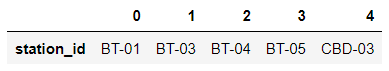
\includegraphics[width = 0.75\textwidth]{1.png}
	\caption{Идентификаторы первых $5$ станций, отсортированных в алфавитном порядке}\label{fig:fig1}
\end{figure}

\begin{figure}[h]
	\centering
	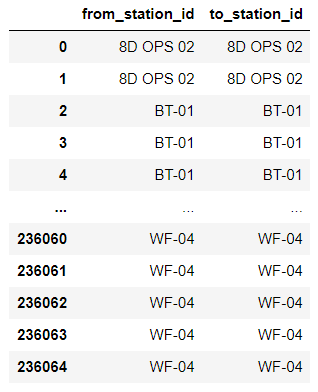
\includegraphics[height = 0.5\textwidth]{2.png}
	\caption{Таблица поездок, отсортированная в алфавитном порядке станций}\label{fig:fig2}
\end{figure}

Здесь возникает несколько проблем с обработкой таблиц. Во-первых, не все станции, которые описаны в столбцах from\_station\_id и to\_station\_id ~\eqref{fig:fig2}, присутствуют в списке station\_id ~\eqref{fig:fig1}. Во-вторых, были такие ячейки столбца to\_station\_id, которые содержали \guillemotleft мусор\guillemotright  \ или не содержали ничего вообще. Эти проблемы будем решать на стадии построения марковской цепи.

\newpage
\section{Алгоритм построения цепи Маркова по таблице данных}

\begin{designation}
	$\letus \, S$~--- множество кодов станций.\\
	$S = \{BT\!-\!01, BT\!-\!03, \ \ldots \ , WF\!-\!04\}$ \\ 
	$N = |S|$~--- количество станций.
\end{designation}

\begin{designation}\label{design:design_dict}
	$\ds{\letus \, d: S \rightarrow \mathds{N}}$~--- словарь кодов станций такой, что
	\begin{align*}
	d("BT\!&-\!01") = 0 \\
	d("BT\!&-\!03") = 1 \\
	&\cdots \\
	d("WF\!&-\!04") = 57 
	\end{align*}
\end{designation}

\begin{designation}
	Под поездкой будем подразумевать упорядоченную пару $(s_{start}, s_{end})$, где $s_{start}$~--- код станции старта, $s_{end}$~--- код станции финиша, $s_{start}, s_{end} \in S$. \\
	Тогда множество $t_n = \left\{ (s_{start_i}, s_{end_i}) \ | \ s_{start_i}, s_{end_i} \in S, \ i \in \{0, \ \ldots, n\} \right\}$~--- таблица поездок размера $n$.
\end{designation}

Марковская цепь, основанная на таблице даннных, строится следующим образом: за переходные состояния принимаем станции, откуда выезжали велосипедисты. А сумма поездок из станции $s_i$ в станцию $s_j$, деленная на общее количество поездок из станции $s_i$, как раз дает нам вероятность попасть из станции $s_i$ в станцию $s_j$ для случайного велосипедиста, $s_i, s_j \in S \ \forall i, j \in \{0, \ \ldots, N\}$.

Чтобы построить Марковскую цепь, необходимо создать словарь $d$~\eqref{design:design_dict}, который идентификаторам станций из таблицы будет сопоставлять число (индекс строки/столбца ячейки переходной матрицы).

С проблемой того, что в столбце $to\_station\_id$ может находиться непонятно что, справляемся следующим образом: пробегаем по списку всех поездок, если не получилось взять значение по ключу словаря $d$, значит поездка состоит из \guillemotleft мусора\guillemotright и мы её обнуляем, в дальнейшем не используя для построения Марковской Цепи.

\begin{designation}\label{design:design1}
	$\letus \, M: N\times N \rightarrow \mathds{N}$~--- матрица, в каждой ячейке которой стоит количество поездок из $s_i$ в $s_j$ в таблице поездок $t_n$. \\
	$M_{ij} = \sum\limits_{\substack{n \geq k \geq 1, \\ d(s_{start_k}) = i, \\ d(s_{end_k}) = j}}{1}$, где $(s_{start_k}, s_{end_k}) \in t_n$.
\end{designation}

\begin{designation}\label{design:design2}
	$\letus \, P_{ij} = \frac{M_{ij}}{\sum\limits_{j = 0}^{N - 1}{M_{ij}}}$~--- отнормированная по строкам матрица $M_{ij}$.\\
	Так как $\forall i \in \left\{ 0, 1, \ \ldots, N - 1\right\}: \sum\limits_{j=0}^{N - 1}(P_{ij}) = 1$, то $P_{ij}$~--- построенная по таблице $t_n$ матрица переходных вероятностей, в каждой ячейке $(i, j)$ которой стоит вероятность попасть из станции $s_i$ в станцию $s_j$, $i, j \in \left\{ 0, 1, \ \ldots, N - 1\right\}$. 
\end{designation}

В нашем случае $N = 58$, $n = 236044$. \\
Для построения матрицы переходных вероятностей $P$~\eqref{eq:eq2} пробегаем по таблице поездок и строим матрицу $M$~\eqref{design:design1}, в каждой ячейке которой стоит количество поездок, совершенных из станции $s_i$ в станцию $s_j$, где $(i, j)$~--- индексы ячейки матрицы.
Далее отнормировав каждую строку матрицы $M$ получаем матрицу $P$, в каждой ячейке которой стоит вероятность попасть из станции $s_i$ в станцию $s_j$, где $(i, j)$~--- индексы ячейки матрицы. Таким образом мы получили матрицу переходных вероятностей~\eqref{fig:fig3} и построили Марковскую цепь~\eqref{eq:eq1}.

\newpage

\begin{figure}[h]
    \centering
    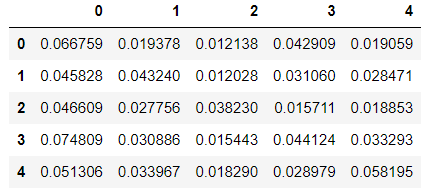
\includegraphics[width = 0.6\textwidth]{3.png}
    \begin{caption}
    	\centering{Вероятности попасть из первых $5$ станций в первые $5$ станций в получившейся матрице переходных вероятностей} \label{fig:fig3}
    \end{caption}
\end{figure}

\chapter{Генерация новых наблюдений и построение цепи Маркова по новым наблюдениям}
\section{Выбор начального состояния}
Для начала нужно определиться, с какой станции мы будем начинать генерацию новых данных. Для этого построим вектор $nss$ размерности $N$ такой, что $nss_i = \sum\limits_{j = 0}^{N-1}{M_{ij}}$. То есть в каждой $i$-ой ячейке находится сумма всех исходящих поездок из станции $s_i$. Отнормировав вектор $nss$ получим вектор $pss = \frac{nss}{||nss||_{1}}$, в каждой $i$-ой ячейке которого будет стоять вероятность начать поездку в станции $s_i$.

\section{Генерация поездок в новой таблице данных}
Будем генерировать $10.000.000$ поездок. Для этого создадим новую матрицу $P_{new}$, изначально заполненную нулями, и новую таблицу $t'_{10.000.000}$~\eqref{fig:fig5} со столбцами $station\_start$ и $station\_end$. $k$-ую поездку в таблице $t'_{10.000.000}$ будем обозначать упорядоченной парой $(s_{start_k}, s_{end_k})$, где $s_{start_k}, s_{end_k}\in S, \ k \in \{1, 2, \ \ldots, 10.000.000\}$.

\begin{mydef}\label{eq:eq3}
	Функция $\xi: \Omega \rightarrow X$ называется случайной величиной, если для любого борелевского множества $B \in \mathfrak{B}(X)$ множество $\xi^{-1}(B)$ является событием, т.е. принадлежит $\sigma$-алгебре $\mathfrak{F}$.
\end{mydef}
\begin{designation}
	$\letus \, \Omega = \left\{0, 1, \ \ldots, N-1\right\}$, случайная величина $\xi: \Omega \rightarrow S$ такая, что $\xi(\omega) = d^{-1}(\omega) \ \forall \omega \in \Omega$~\eqref{eq:eq3}, и\\
	\begin{table}[h]
		\begin{center}
			\begin{tabular}{|c|c|c|c|c|c|}
				\hline
				$\xi$	&	$BT\!-\!01$	&	$BT\!-\!03$	&	$BT\!-\!04$	&	$\ldots$	&	$WF\!-\!04$ \\ \hline
				$P$	&	$pss_0$	&	$pss_1$	&	$pss_2$	&	$\ldots$	&	$pss_{N-1}$ \\ \hline
			\end{tabular}
		\end{center}
		\caption{Распределение случайной величины $\xi$}\label{table:table1}
	\end{table}
\end{designation}

Выберем случайную начальную станцию $s_{initial}$, с которой будем стартовать генерацию, по вероятности из вектора $pss$, то есть по распределению случайной величины $\xi$. Запишем её в таблицу данных. Таким образом $s_{start_1} = s_{initial} = \xi$.

\begin{designation}
	$\letus \, \Omega = \left\{0, 1, \ \ldots, N-1\right\}, \ \forall i \in \Omega:$ случайная величина $\eta_i: \Omega \rightarrow S$ такая, что $\eta_i(\omega) = d^{-1}(\omega) \ \forall \omega \in \Omega$~\eqref{eq:eq3}, и
	\begin{table}[h]
		\begin{center}
			\begin{tabular}{|c|c|c|c|c|c|}
				\hline
				$\eta$	&	$BT\!-\!01$	&	$BT\!-\!03$	&	$BT\!-\!04$	&	$\ldots$	&	$WF\!-\!04$ \\ \hline
				$P$	&	$P_{i_0}$	&	$P_{i_1}$	&	$P_{i_2}$	&	$\ldots$	&	$P_{i_{N-1}}$ \\ \hline
			\end{tabular}
		\end{center}
		\caption{Распределение случайной величины $\eta_i$}\label{table:table1}
	\end{table}
\end{designation}

Далее выберем случайную следующую станцию $s_{end_1}$ по вероятности из вектора $P_i$, то есть по распределению случайной величины $\eta_i$, где $i = d(s_{start_1})$, запишем её в таблицу. Первая поездка таблицы $t'_{10.000.000}$ равна $\left(s_{start_1}, s_{end_1}\right)$. Следующая поездка будет начинаться из станции $s_{end_1}$, таким образом $s_{start_2} = s_{end_1}$. Продолжаем генерировать следующие поездки: $s_{end_i} = \eta_{d(s_{start_i})}, \ s_{start_i} = s_{end_{i-1}}, \ i = 1 \ldots 10.000.000$.

\section{Построение новой цепи Маркова по сгенерированным поездкам}
Параллельно с генерацией поездок строим матрицу $M_{new}$, в каждой ячейке которой стоит количество поездок из $s_i$ в $s_j$ в таблице поездок $t'_{10.000.000}$, по аналогии с матрицей $M$~\eqref{design:design1}.

\begin{mydef}\label{eq:eq4}
	В пространстве m-мерных векторов $R^m$ введена фиксированная норма $||x||$ (например, одна из норм $||x||_p$, $1 \leq p \leq \infty$, в зависимости от того, какая ошибка нам нужна: линейная, среднеквадратичная и т.п.). В этом случае в качестве меры степени близости векторов $x$ и $x^{*}$ естественно использовать величину $||x - x^{*}||$, являющуюся аналогом расстояния между точками $x$ и $x^{*}$. \\ Введём абсолютную и относительную ошибки вектора $x^{*}$ с помощью формул:
	\begin{equation*}
		\Delta\left(x^{*}\right) = ||x - x^{*}||, \  \delta\left(x^{*}\right) = \frac{||x - x^{*}||}{||x||}. 
	\end{equation*}
\end{mydef}

\begin{mydef}\label{eq:eq5}
	Нормой матрицы $A$ называется величина $||A|| = \underset{x \neq 0}{max}\frac{||Ax||}{||x||}$. \\
	Абсолютная и относительная погрешности матрицы вводятся аналогично погрешностям вектора с помощью формул:
	\begin{equation*}
		\Delta\left(A^{*}\right) = ||A - A^{*}||, \
		\delta\left(A^{*}\right) = \frac{||A - A^{*}||}{||A||}.
	\end{equation*}
\end{mydef}

Через каждое количество поездок, кратное порядку $10$, начиная с $10.000$ и до $10.000.000$, нормируем по строкам матрицу $M_{new}$, таким образом получаем матрицу $P_{new}$~\eqref{fig:fig4} по аналогии с получением матрицы переходных вероятностей $P$ из матрицы $M$~\eqref{design:design2} и считаем абсолютную и относительную ошибки по формуле~\eqref{eq:eq5}, где $A$~--- начальная матрица переходных вероятностей $P$, $A^{*}$~--- новая матрица $P_{new}$, построенная на сгенерированных данных.

\begin{figure}[h]
	\begin{subfigure}{0.5\textwidth}
    		\centering
    		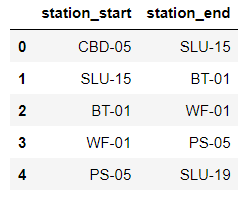
\includegraphics[width = 0.9\linewidth]{5.png}
		\begin{caption}
    			\centering{Первые $5$ строк в таблице сгенерированных данных $t'$} \label{fig:fig5}
    		\end{caption}
	\end{subfigure}
	\begin{subfigure}{0.5\textwidth}
    		\centering
    		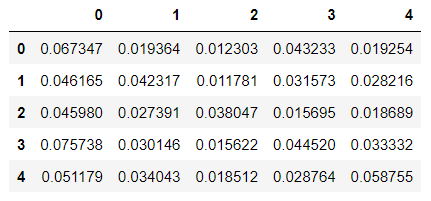
\includegraphics[width = 0.9\linewidth]{4.png}
    		\begin{caption}
    			\centering{Вероятности попасть из первых $5$ станций в первые $5$ станций в новой построенной по сгенерированным данным матрице переходных вероятностей $P_{new}$} \label{fig:fig4}
    		\end{caption}
		\end{subfigure}
\end{figure}

\chapter{Сравнение двух цепей Маркова}

Программа выдала следующие результаты:

\begin{table}[h]
	\begin{center}
		\begin{tabular}{|c|c|c|}
			\hline
   			Количество поездок		& Абсолютная погрешность	& Относительная погрешность  \\ \hline
			10.000 & 0.895783 & 0.439285 \\ \hline
			100.000 & 0.277931 & 0.136295 \\ \hline
			1.000.000 & 0.092052 & 0.045583 \\ \hline
			10.000.000 & 0.026711 & 0.013099 \\ \hline
		\end{tabular}
	\end{center}
	\caption{Абсолютные и относительные погрешности рассчетов}\label{table:table2}
\end{table}

В учебном пособии по теории вероятностей~\cite[Гл. 8]{Chernova} вводится следующая теорема: 
\begin{theorem}[Центральная предельная теорема Ляпунова]\label{theo:theo_CPT}
	 \\
	$\letus \ \xi_1, \xi_2,\ldots$~--- независимые и одинаково распределённые случайные величины с конечной и ненулевой дисперсией: $0 < \mathbf{D}\xi_1 < +\infty$. $S_n = \xi_1 + \ldots + \xi_n$. Тогда имеет место слабая сходимость
	\begin{equation}
		\frac{S_n - n \mathbf{E}\xi_1}{\sqrt{n \mathbf{D}\xi_1}} \Rightarrow N_{0, 1}
	\end{equation}
	
	Откуда не трудно вывести соотношение:
	\begin{equation}
		P \left( \left| \frac{1}{n} \sum\limits_{i = 1}^n{\xi_i} - \mathbf{E}\xi_1 \right| \leq k \frac{\sqrt{\mathbf{D}\xi_1}}{\sqrt{n}} \right) \Rightarrow 2\Phi(k) - 1
	\end{equation}
	
	Заметим, что для больших $n$, при увеличении $n$ отклонение $\left| \frac{1}{n} \sum\limits_{i = 1}^n{\xi_i} - \mathbf{E}\xi_1 \right|$ уменьшается в $\sqrt{n}$ раз.
\end{theorem}

Как мы видим~\eqref{table:table2}, при увеличении числа поездок в $100$ раз абсолютная и относительная погрешности уменьшаются примерно в $10$ раз. Значит ошибки обратно пропорциональны корню из количества поездок. Ссылаясь на центральную предельную теорему~\eqref{theo:theo_CPT} и принимая во внимание тот факт, что в нашем случае можем считать каждый элемент матрицы $P_{new}$ преобразованием величин $\xi$ и $\eta_i$, а каждый элемент матрицы $P$~--- математическим ожиданием этого преобразования, можем заключить, что изначально построенная матрица переходных вероятностей $P$ построена корректно.

\chapter{Следующая задача}

Следующей задачей я ставлю рассчет матрицы первых достижений по новой матрице переходных вероятностей Марковской цепи, построенной на сгенерированных данных, и проверку корректности её значений с помощью алгоритма подсчёта времен первых достижений через таблицу сгенерированных данных.










 

\bibliographystyle{ugost2008}

\bibliography{biblio.bib}








 

\end{document}
